\documentclass{sigchi}

% Use this command to override the default ACM copyright statement (e.g. for preprints). 
% Consult the conference website for the camera-ready copyright statement.


%% EXAMPLE BEGIN -- HOW TO OVERRIDE THE DEFAULT COPYRIGHT STRIP -- (July 22, 2013 - Paul Baumann)
\toappear{Permission to make digital or hard copies of all or part of this work for personal or classroom use is 	granted without fee provided that copies are not made or distributed for profit or commercial advantage and that copies bear this notice and the full citation on the first page. Copyrights for components of this work owned by others than ACM must be honored. Abstracting with credit is permitted. To copy otherwise, or republish, to post on servers or to redistribute to lists, requires prior specific permission and/or a fee. Request permissions from permissions@acm.org. \\
 {\emph{CHI'14}}, April 26--May 1, 2014, Toronto, Canada. \\
 Copyright \copyright~2014 ACM ISBN/14/04}
% EXAMPLE END -- HOW TO OVERRIDE THE DEFAULT COPYRIGHT STRIP -- (July 22, 2013 - Paul Baumann)


% Arabic page numbers for submission. 
% Remove this line to eliminate page numbers for the camera ready copy
% \pagenumbering{arabic}


% Load basic packages
\usepackage{balance}  % to better equalize the last page
\usepackage{graphics} % for EPS, load graphicx instead
\usepackage{times}    % comment if you want LaTeX's default font
\usepackage{url}      % llt: nicely formatted URLs

% llt: Define a global style for URLs, rather that the default one
\makeatletter
\def\url@leostyle{%
  \@ifundefined{selectfont}{\def\UrlFont{\sf}}{\def\UrlFont{\small\bf\ttfamily}}}
\makeatother
\urlstyle{leo}


% To make various LaTeX processors do the right thing with page size.
\def\pprw{8.5in}
\def\pprh{11in}
\special{papersize=\pprw,\pprh}
\setlength{\paperwidth}{\pprw}
\setlength{\paperheight}{\pprh}
\setlength{\pdfpagewidth}{\pprw}
\setlength{\pdfpageheight}{\pprh}

% Make sure hyperref comes last of your loaded packages, 
% to give it a fighting chance of not being over-written, 
% since its job is to redefine many LaTeX commands.
\usepackage[pdftex]{hyperref}
\hypersetup{
pdftitle={SIGCHI Conference Proceedings Format},
pdfauthor={LaTeX},
pdfkeywords={SIGCHI, proceedings, archival format},
bookmarksnumbered,
pdfstartview={FitH},
colorlinks,
citecolor=black,
filecolor=black,
linkcolor=black,
urlcolor=black,
breaklinks=true,
}

% create a shortcut to typeset table headings
\newcommand\tabhead[1]{\small\textbf{#1}}


% End of preamble. Here it comes the document.
\begin{document}

\title{Collective Intelligence}

\numberofauthors{1}
\author{
  \alignauthor Jeremy Cole, Jiawei Chen, Ying Xu, Feng Sun\\
    \affaddr{Pennsylvania State University}\\
    \affaddr{College of IST, University Park, PA 16802}\\
    \email{\{jrcole, ,ying.xu, \}}\\
    \affaddr{Optional phone number}
}

\maketitle

\begin{abstract}
In this paper, we give an overview of the theory of Collective Intelligence as it relates to Human-Computer Interaction. To fully cover this theory, we examine three separate descriptions: as an information processing model, as a model for small group task performance, and as a model of tasks at scale. We additionally compare Collective Intelligence to related theories and give a survey of papers in the area.
\end{abstract}

\keywords{
	Collective Intelligence. Theory. Literature Review. \newline
}

\category{H.5.2.}{HCI Theory}{Collective Intelligence}
\section{Introduction}

This format is to be used for submissions that are
published in the conference proceedings.  We wish to give
this volume a consistent, high-quality appearance. We
therefore ask that authors follow some simple
guidelines. In essence, you should format your paper
exactly like this document. The easiest way to do this is
simply to download a template from the conference web
site, and replace the content with your own material.
\section{Classical Collective Intelligence}
In 1990s, John Smith wrote a book called Collective Intelligence in Computer-Based Collaboration which is now considered the classical Collective Intelligence. The book has two main parts: one is the foundation concepts about collective intelligence and its theoretical origin; the other one is about the core ideas in the theory \cite{cibook}. Smith regards collaboration as an information processing activity and computer system as a part of this collaboration system together with human. And key elements in the system that across both computer system and human are Collective Memory, Collective Processing, Collective Strategy and Collective Awareness and Control.

\subsection{Collaboration as an Information Processing Activity}
The work of a group is focused in the production of some concrete product or in problem-solving. Although groups differ significantly in their sies, location, duration, completion of the group mission and the ways the group works, there are surprisingly siginificant similarities among their distributed activities. So as a group, they share a body of knowledge about their work. The ways to share knowledge among group members across time and location, and how to use the knowledge to guide their practices into achieving the goals are the two main questions to look in the theory. In order to find the similarities, Simith examined into different collaboration scenarios to illustrate the range of behaviors commonly found in the collaborative groups, and to describe the informaiton flow from one to another. In summary, groups are all concerned with producing some type of tangible product. All of them produced several types of intangible knowledge, some shared within the group and some kept private. For all the tangible, ingangible and ephemeral konwledge that have been created in the process, they transfer from one form to another form among the group members. Please refer to the figure below.

\begin{figure}[!h]
\centering
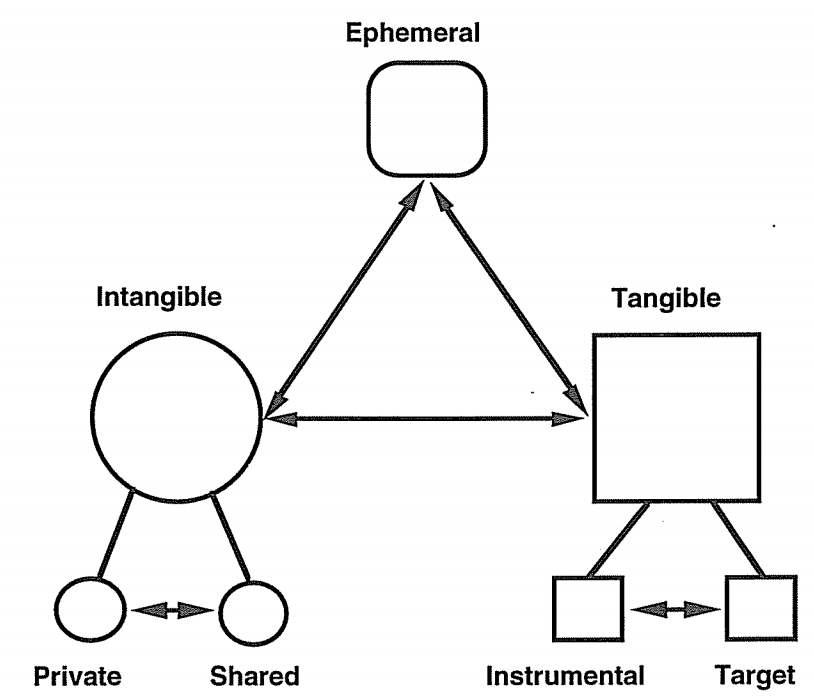
\includegraphics[width=0.9\columnwidth]{figure/IPS}
\caption{Information Types in a Collaboration System}
\label{fig:IPS}
\end{figure}

\subsection{Computer Support for Collaboration}
Collaborative group work requires a variety of tools to facilitate the process. This work focused on computers as the tool to help create knowledge, tranform knowledge and enhance the information flow among different members in the group. In addition to computers, the author also looked into various collabroative softwares - both synchronous and asynchronous - in the support of independent work and collaborative work. Some asychronous tools include email, FTP, Network File Systems and so on. Synchronous tools like audio/video conferencing was also examined in the work. Smith also proposed a comprehensive system for collaboration, showed in the following figure. Three workstations are connected to a hypermedia storage system and to one another by a high-speed network. The same conferenced brower can be seen on each workstation, with supporting video window. 

\begin{figure}[!h]
\centering
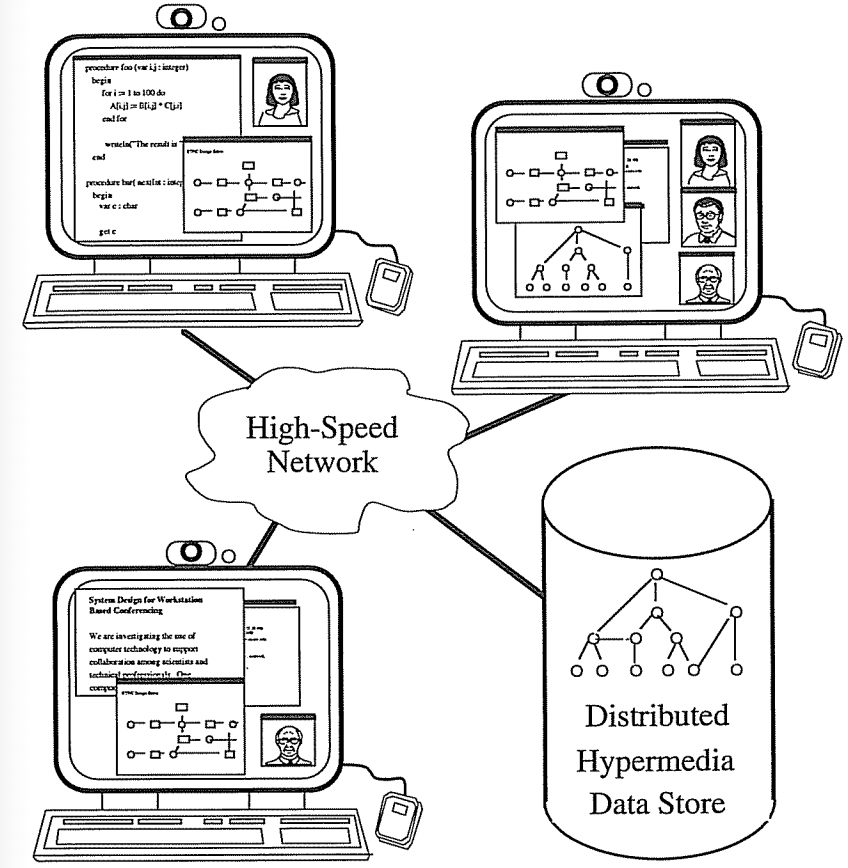
\includegraphics[width=0.9\columnwidth]{figure/ABC}
\caption{Artifact-Based Collaboration System}
\label{fig:ABC}
\end{figure}

\subsection{Concepts of Collective Intelligence}
There are four identified in the collective intelligence system shared with human and computer: collective memory, processing, strategy and awareness/control.

\subsubsection{Collective Memory}
In this collaborative system, memory systems provide the storage of both long-term and short-term memories. Additionally to the storage, the constructs that function as a form of collective memory for the group is also examined. It includes provisions for the long-term storage and retrieval of information, analogous to human long-term memory, and it provides contexts in which that information can be activated and processed, analogous to working memory. 

\subsubsection{Collective Processing}
Collective processing focuses on the form and function of individual small-grained processes that operate in the contexts identified as the group's working memory. They are responsible for basic actions such as retrieving and defining concepts, identifying relationships, building conceptual structures, making changes to those structures and storing results. In this way, it enables the group to function as an information processing system and reach the goal of the group.

\subsubsection{Collective Strategy}
Strategy, on the other hand, extends its scope beyond individually independent entities and processing and considers the relation between one and another. The focus is on the patterns in the sequences of processes that occur in the behavior of a group. By engaging processes not as isolated actions but in coherent sequences, groups are able to function in purposeful ways and to accomplish goals.

\subsubsection{Awareness and Control}
The work talks about two metacognitive issues - awareness and control. Awareness plays a large role in enabling an individual to produce intellectual products that are coherent and internally consistent. It also examines the ways in which a group can piece together partial, but overlapping bodies of knowledge among its members to produce partial but overlapping fields of awareness.

Authority and administrative control wihtin groups in relation to issues of self-controal in individuals are also important part of the discussion. A balance between delegated and centralized authority is needed to motivate groups and to enable them to produce work with intellectual integrity.

























\section{Small-scale CI}
Similar to \lq general intelligence\rq ~\cite{deary2000looking} which indicates the charactieristic levels of intelligence for individuals, researchers ~\cite{science} have studied and shown that there exists a single statistical factor \lq c factor\rq : the \lq collective intelligence\rq that could explain the performance of small groups (e.g. two to five people) on a wide range of tasks. A group's collective intelligence infers that a group's ability to perform one task is correlated with its ability to perform a wide range of other tasks ~\cite{science}. Empirically, the average inter-item correlation for group scores on different tasks is positive, and there is a factor extracted in the factor analysis of these scores which accounts for 30$\%$ to 50$\%$ of the variance, while the following factors account for substantially less variance ~\cite{science}. 

In ~\cite{science}, the authors first support the existance of such a general collective intelligence factor by demonstrating their results with two studies. The first study envolves 40 three-person groups working on tasks from the McGrath Task Circumplex ~\cite{mcgrath1984groups} and the results positively support the authors' hypothesis. The collective intelligence factor also has significant effect when predicting the performance on the criterion task, while the average individual intelligence and the maximum individual intelligence do not. In the second study, the authors use 152 groups ranging from 2 to 5 peopleand 5 additional tasks in order to replicate their findings in groups of different sizes and a broader sample of tasks. As expected, the results again supported the existance of a general collective intelligence factor.

The authors in ~\cite{science} also find out three main facots that cause the collective intelligence factor. First, collective intelligence is significantly correlated with the average social sensitivity of group members. Second, groups where the the conversation is dominated by fewer peope has less collective intelligence. Third, their results show that the c factor is positively and significantly correlated with the proportion of females group members. However, this find largely overlaps with the first finding as women in their study have better score on social sensitivity.

The findings in ~\cite{science} show that collective intelligence depend both on the properties of the group (such as the average intelligence of group members) and on how the groups members interact with each other. These findings open the door to many important research questions to raise the intelligence of a group as a whole rather than on the individual scale. 

\section{Sections}

The heading of a section should be in Helvetica 9-point bold, all in
capitals. Use Arial if Helvetica is not available. Sections should
not be numbered.

\subsection{Subsections}

Headings of subsections should be in Helvetica 9-point bold with
initial letters capitalized.  For
sub-sections and sub-subsections, a word like \emph{the} or \emph{of}
is not capitalized unless it is the first word of the heading.)

\subsubsection{Sub-subsections}

Headings for sub-subsections should be in Helvetica 9-point italic
with initial letters capitalized.  Standard {\textbackslash}section,
{\textbackslash}subsection, and {\textbackslash}subsubsection commands
will work fine.
\section{Drawbacks}

\subsection{Scope}

Collective Intelligence has been applied outside of simple information processing; however, its applications are generally limited to tasks where the participants have relatively low communication. Even if communication is technically involved, it is relatively cursory and task-oriented. Real social interaction is not really included.

Further, entrenched social factors are not really included. This means that while collective intelligence might be a good level of analysis for an idealized group, or for a general group, it may miss a lot of the detail involved in a specific group. While a group may behave like a general group at certain times in toy tasks, in a workplace, where social relations and common practice have built up over years, they are likely to have many factors that are not covered by the theory. 

This makes the scope of Collective Intelligence to at least partially be restricted to toy tasks. Of course, with the advent of crowdsourcing, toy tasks with little communication and very little complicated social factors are very common. 

\subsection{Ethical}

From an ethical standpoint, the types of tasks that Collective Intelligence is often interested in (crowdsourcing) has a few dilemmas. In directed crowdsourcing, as discussed earlier, workers are recruited for small amounts of money to perform simple tasks. Normally, they are paid based on task completion, rather than an hourly wage, which allows this type of work to avoid minimum wage laws. This places the workers who complete such tasks in a similar group as migrant farmworkers or sweatshop workers. However, since the tasks are often over the Internet, this problem may not render itself apparent to the organizer of the task: he or she likely never even meets the people working for him or her. 

On the other side of the spectrum, the types of tasks involved in passive crowdsourcing offer different kinds of problems. While the data is hopefully not individually identifiable, it is still data that is being collected for use in some type of research. Most likely, this is done without the user's consent and the user is also not compensated. While the controversial Facebook study had experimental manipulation \cite{facebook1}, there has been controversy over researchers that simply used publicly generated data \cite{facebook2}. While this problem is not limited to Collective Intelligence, it is applicable to many types of CI-at-scale research.  

\subsection{Cognitive}

While Collective Intelligence theoretically could make use of the full range of the cognitive capabilities of a human, that is generally not the case. Many crowdsourcing tasks rely on fairly rote procedures. For instance, the Find-Fix-Verify paradigm discussed earlier takes the complex task of writing and breaks it into tasks that are fairly simple on their own. Then, it has each person perform one of these fairly simple tasks. Other common tasks, such as image labeling, have each person perform a task that even algorithms can generally perform correctly. In few of the tasks, the full power of human cognitive abilities is used.

Paradigms like ACT-R \cite{actr} generally rely on people's innate ability to learn. While simpler formulations have been criticized as only modeling expert behavior, the cognitive paradigm has largely moved beyond that. Collective Intelligence as a theory, however, is largely rooted in the same type of toy tasks that make up IQ tests. These tasks generally are designed such that learning has little or no effect, because the goal is for a person's IQ score to remain more or less constant, regardless of their experience. However, this construction ignores one of the most fundamentally powerful pieces of human intelligence. 
\section{Application 1: }
Fill in here (~1 page)! Jiawei
\section{Language, Style and Content}

The written and spoken language of SIGCHI is English. Spelling and
punctuation may use any dialect of English (e.g., British, Canadian,
US, etc.) provided this is done consistently. Hyphenation is
optional. To ensure suitability for an international audience, please
pay attention to the following:

\begin{itemize}
\item Write in a straightforward style.
\item Try to avoid long or complex sentence structures.
\item Briefly define or explain all technical terms that may be
  unfamiliar to readers.
\item Explain all acronyms the first time they are used in your text---e.g.,
``Digital Signal Processing (DSP)''.
\item Explain local references (e.g., not everyone knows all city
  names in a particular country).
\item Explain ``insider'' comments. Ensure that your whole audience
  understands any reference whose meaning you do not describe (e.g.,
  do not assume that everyone has used a Macintosh or a particular
  application).
\item Explain colloquial language and puns. Understanding phrases like
  ``red herring'' may require a local knowledge of English.  Humor and
  irony are difficult to translate.
\item Use unambiguous forms for culturally localized concepts, such as
  times, dates, currencies and numbers (e.g., ``1-5-97'' or ``5/1/97''
  may mean 5 January or 1 May, and ``seven o'clock'' may mean 7:00 am or
  19:00).  For currencies, indicate equivalences---e.g., ``Participants
  were paid 10,000 lire, or roughly \$5.''
\item Be careful with the use of gender-specific pronouns (he, she)
  and other gendered words (chairman, manpower, man-months). Use
  inclusive language that is gender-neutral (e.g., she or he, they,
  s/he, chair, staff, staff-hours,
  person-years). See~\cite{Schwartz:1995:GBF} for further advice and
  examples regarding gender and other personal attributes.
\item If possible, use the full (extended) alphabetic character set
  for names of persons, institutions, and places (e.g.,
  Gr{\o}nb{\ae}k, Lafreni\'ere, S\'anchez, Universit{\"a}t,
  Wei{\ss}enbach, Z{\"u}llighoven, \r{A}rhus, etc.).  These characters
  are already included in most versions of Times, Helvetica, and Arial
  fonts.
\end{itemize}
\section{Theory Police}
The concept of Collective Intelligence itself has been around for thousands of years since people work, make decisions, and collaborate together in the form of families and communities. However, with the increasing advancement, spreading and adoption of information technologies and Internet, the idea of collective intelligence changes dramatically. In small scale, people are working together in labs, collaborating remotely through real time applications, and in other forms. Many study towards this direction look at how to improve the efficiency of information sharing, how to tranform implicit knowledge into explicit one, and how to reach the goal of problem-solving or product creation more effectively for the group as a whole. In large scale examples of collective intelligence, people look at crowdsourcing in differnet domains like finance, citizen science and knowledge creation. Even though collective intelligence at scale is heavily focusing on the crowdsourcing, we do not have a integrated definition towards the meaning of crowdsourcing. So in the theory police part, first, we are examining the integrated definition of it.

\subsection{Integrated Definition of Crowdsourcing}
The work we refer to is called Towards an Integrated Crowdsourcing defnition by Enrique Estelles-Aroles and Fernando Gonzalez-Ladron-de-Guevara. The problem they see in the field is that the diversity of crowdsourcing applications leads to the blurring of the limits of crowdsourcing, which could be identified virtually with any type of internet-based collaborative activity. Thus, The paper used literature review as research method to find an validated exhaustive definition of crowdsourcing. By doing so, first, it follows the Tatarkiewicz's approach to include all the paper that relate to crowdsourcing and all the elements whose characteristics differentiate crowdsourcing from other collaborative activities based on ICT. Second, it borrows Vukovic and Aliabarian's view to check the validity of the definition. In the end, it presents its findings of three main elements in the definition of crowdsourcing which are crowd, initiator and process. Crowd has three characterisitcs, which are who forms it; what it has to do; and what it gets in return. For initiator, it has to answer two question: who it is; and what they get in return for the work of the crowd. For process, the type of process; the type of call used; and the medium used are the three main features to identify\cite{theorypolice1}.

\subsection{Differences With Distributed Cognition}
We naturally link Collective Intelligence theory with Distributed Cognition theory for the similarities they share. For example, they both study groups; they both have a specific goal to achieve: either problem-solving or product creation; and they all have three main elements in their theory: group of people, problems/goals and tools. But also they have significant differences to distinguish with each other.

First, they have different origin. Distributed Cognition is coming from psychology. It studies how groups coordinate their behaviors with each other. It treats group work as cognitive problems because the system exhibits purposeful behaviors in problem solving and information processing\cite{dcog}. Collective Intelligence is more commonly found in management science and organizational study. 

Second, Distribted Cognition could be used to discover social and cultural dimensions of work, relating these back to system development and HCI. However, the relationship between Collective Intelligence with HCI is not as directly applied as DCog with HCI.

Third, the sizes of groups on which these two theories study are different from each other. Collective Intelligence has a broader scope of groups, which ranges from small 2-5 member groups to thousands people from crowdsourcing applications. However, DCog is applied in much smaller groups than Collective Intelligence.

Forth, Distributed Cognition is a more closed system than Collective Intelligence. The following figure shows that DCog system has its input and output, and in between there are human-computer representations and the processes between them. Like cognitive system, Dcog has
its information processing activities but with both human minds and computers. But for Collective Intelligence, we do not see this clear and closed system developed yet.

\begin{figure}[!h]
\centering
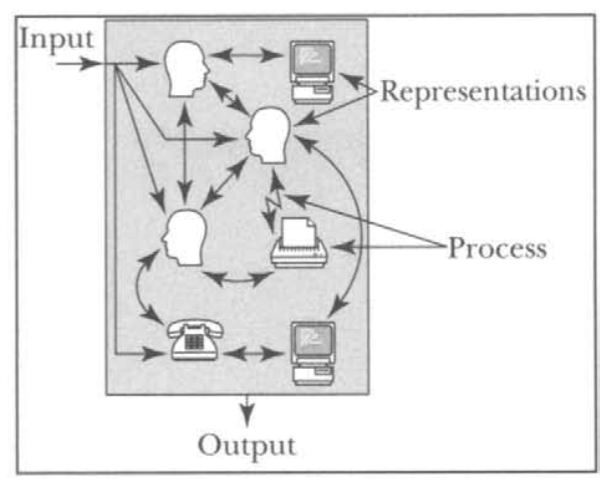
\includegraphics[width=0.9\columnwidth]{figure/DCog}
\caption{Distributed Cognition System}
\label{fig:Dcog}
\end{figure}




\section{Conclusion}
In this review, we have covered the evolving viewpoint of the theory of Collective Intelligence and its applications. The Collective Intelligence theory began as a methodology to study classical information processing, modeling a group of people as a distributed computer. It later became a way to discuss a method of measurement for general intelligence of a group of people, in a similar way to how the IQ test formalized this idea for a single person. Later, it became a method for analyzing intelligence at scale: how to get good results out of a large number of people performing a task. We have went through two applications, mostly viewing CI in this latter sense, the WikiCrimes system and a rating system. 

There are some criticisms of the theory from two standpoints. From a theoretical standpoint, it does not seem to say very much that distributed cognition does not, and it's unclear what exactly crowdsourcing is, depending on who's talking. From an application standpoint, the theory suffers from ethical dilemmas, is limited in scope, and fails to consider the full capability of humans.

These criticisms are only partially valid on the actual applications we presented. Both to an extent involve relatively complicated tasks, and especially with the WikiCrimes system, possible benefits to the users. In a sense, this is because the WikiCrimes system is a collaborative crowdsourcing platform instead of a directed crowdsourcing platform. However, we still contend neither of these applications make use of people's ability to learn, which is fundamental to human intelligence. 

With the rise of MOOCs in popularity and the massive amount of unlabeled data that can now be collected, Collective Intelligence is in a good position for application in the future in the fields of CSCW and HCI.


% Balancing columns in a ref list is a bit of a pain because you
% either use a hack like flushend or balance, or manually insert
% a column break.  http://www.tex.ac.uk/cgi-bin/texfaq2html?label=balance
% multicols doesn't work because we're already in two-column mode,
% and flushend isn't awesome, so I choose balance.  See this
% for more info: http://cs.brown.edu/system/software/latex/doc/balance.pdf
%
% Note that in a perfect world balance wants to be in the first
% column of the last page.
%
% If balance doesn't work for you, you can remove that and
% hard-code a column break into the bbl file right before you
% submit:
%
% http://stackoverflow.com/questions/2149854/how-to-manually-equalize-columns-
% in-an-ieee-paper-if-using-bibtex
%
% Or, just remove \balance and give up on balancing the last page.
%
\balance

\bibliographystyle{acm-sigchi}
\bibliography{collect-int}
\end{document}
